\achapter{12}{The Structure of $\R^n$} \label{chap:R_n}

\vspace*{-17 pt}
\framebox{
\parbox{\dimexpr\linewidth-3\fboxsep-3\fboxrule}
{\begin{fqs}
\item What properties make $\R^n$ a vector space?
\item What is a subspace of $\R^n$?
\item What properties do we need to verify to show that a set of vectors is a subspace of $\R^n$? Why?
\item What important structure does the span of a set of vectors in $\R^n$ have?  
%\item What is an eigenspace of a matrix? 
\end{fqs}}}% \hspace*{3 pt}}

\vspace*{13 pt}

\csection{Application: Connecting GDP and Consumption in Romania}
\label{sec:appl_romania}

It is common practice in the sciences to run experiments and collect data. Once data is collected it is necessary to find some way to analyze the data and predict future behavior from the data. One method is to find a curve that best ``fits" the data, and one widely used method for curve fitting is called the \emph{least squares} method.

For example, economists are often interested in \emph{consumption}, which is the purchase of goods and services for use by households. In ``A Statistical Analysis of GDP and Final Consumption Using Simple Linear Regression, the Case of Romania 1990-2010",\footnote{B\u{a}l\u{a}cescu, Aniela \& Zaharia, Marian. (2012). A STATISTICAL ANALYSIS OF GDP AND FINAL CONSUMPTION USING SIMPLE LINEAR REGRESSION. THE CASE OF ROMANIA 1990?2010. Annals - Economy Series. 4. 26-31. Available from: \url{https://www.researchgate.net/publication/227382939_A_STATISTICAL_ANALYSIS_OF_GDP_AND_FINAL_CONSUMPTION_USING_SIMPLE_LINEAR_REGRESSION_THE_CASE_OF_ROMANIA_1990-2010}.} the authors collect data and then use simple linear regression to compare GDP (gross domestic product) to consumption in Romania. The data they used is seen in Table \ref{T:GDP_consumption}, with a corresponding scatterplot of the data (with consumption as independent variable and GDP as dependent variable). The units for GDP and consumption are milliions of leu (the currency of Romania is the leu -- on December 21, 2018, one leu was worth approximately \$0.25 U.S.)
The authors conclude their paper with the following statement: 
\begin{quote}
``However, we can appreciate that linear regression model describes the correlation between the value of gross domestic product and the value of final consumption and may be transcribed following form: 
\begin{center} PIB = -3127.51+ 1.22 CF. \end{center}

Analysis of correlation between GDP and final consumption (private consumption and public consumption) will result in an increase of 1.22 units of monetary value of gross domestic product. 
 
We can conclude that the Gross Domestic Product of our country is strongly influenced by the private and public consumption."
 \end{quote}

\begin{figure}[ht]
\begin{center}
\begin{minipage}{1.75in}
\begin{center}
\setlength{\tabcolsep}{2pt}
\hspace{-0.5in} \begin{tabular}{ccc} \hline
Year		&\hspace{0.2in} GDP \hspace{0.2in}		&Consumption \\ \hline
$1990$ 	&$85.8$ 		&$68.0$ \\ \hline
$1991$ 	&$220.4$ 		&$167.3$ \\ \hline
$1992$ 	&$602.9$ 		&$464.3$ \\ \hline
$1993$ 	&$2003.9$ 	&$1523.6$ \\ \hline
$1994$ 	&$4977.3$	&$3845.2$ \\ \hline
$1995$ 	&$7648.9$	&$6257.7$ \\ \hline
$1996$ 	&$11384.2$ 	&$9713.8$ \\ \hline
$1997$ 	&$25529.8$	&$ 21972.2$ \\ \hline
$1998$ 	&$37055.1$ 	&$33311.2$ \\ \hline
$1999$ 	&$55191.4$	&$49311.9$ \\ \hline
$2000$ 	&$80984.6$ 	&$69587.4$  \\ \hline
$2001$ 	&$117945.8$ 	&$100731.7$ \\ \hline
$2002$ 	&$152017.0$ 	&$127118.8$ \\ \hline
$2003$	&$197427.6$ 	&$168818.7$ \\ \hline
$2004$  	&$247368.0$ 	&$211054.6$ \\ \hline
$2005$ 	&$288954.6$  	&$251038.1$ \\ \hline
$2006$  	&$344650.6$  	&$294867.6$  \\ \hline
$2007$  	&$416006.8$  	&$344937.0$ \\ \hline
$2008$  	&$514700.0$  	&$420917.5$ \\ \hline
$2009$  	&$498007.5$  	&$402246.0$ \\ \hline 
$2010$  	&$513640.8$  	&$405422.4$ \\ \hline  
\end{tabular}
\captionof{table}{GDP and consumption in Romania.}
\label{T:GDP_consumption}
\end{center}
\end{minipage} \hspace{0.25in}
\begin{minipage}{2.0in}
\begin{center}
\resizebox{!}{2.0in}{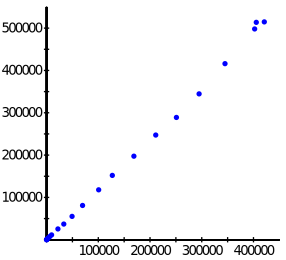
\includegraphics{GDP_consumption}}
\end{center}
\captionof{figure}{GDP and consumption data plot.}
\label{F:GDP_consumption}
\end{minipage}
\end{center}
\end{figure}


As we can see from the scatterplot, the relationship between the GDP and consumption is not exactly linear, but looks to be very close. To make correlations between GDP and consumption as the authors did, we need to understand how they determined their approximate linear relationship between the variables.  With a good approximation function we can then compare the variables, extrapolate from the data, and make predictions or interpolate and estimate between data points. For example, we could use our approximation function to predict, as the authors did, how changes in consumption affect GDP (or vice versa). Later in this section we will see how to find the least squares line to fit this data -- the best linear approximation to the data. This involves finding a vector in a certain subspace of $\R^2$ that is closest to a given vector. Linear least squares approximation is a special case of a more general process that we will encounter in later sections where we learn how to project sets onto subspaces. 


\csection{Introduction}
\label{sec:rn_intro}

The set $\R^n$ with vector addition and scalar multiplication has a nice algebraic structure. These operations satisfy a number of properties, such as associativity and commutativity of vector addition, the existence of an additive identity and additive inverse, distribution of scalar multiplication over vector addition, and others. These properties make it easier to work with the whole space since we can express the vectors as linear combinations of basis vectors in a unique way. This algebraic structure makes $\R^n$ a \emph{vector space}. 

There are many subsets of $\R^n$ that have this same structure. These subsets are called \emph{subspaces} of $\R^n$. These are the sets of vectors for which the addition of any two vectors is defined within the set, the scalar multiple of any vector by any scalar is defined within the set and the set contains the zero vector. One type of subset with this structure is the span of a set of vectors. 
 
Recall that the span of a set of vectors $\{\vv_1, \vv_2, \ldots, \vv_k\}$ in $\R^n$ is the set of all linear combinations of the vectors. For example, if $\vv_1=\left[ \begin{array}{c} 1\\1\\0\end{array} \right]$ and $\vv_2=\left[ \begin{array}{c} 1\\0\\1\end{array} \right]$, then a linear combination of these two vectors is of the form
\[ c_1 \vv_1 + c_2 \vv_2 = c_1 \left[ \begin{array}{c} 1\\1\\0\end{array} \right] + c_2 \left[ \begin{array}{c} 1\\0\\1\end{array} \right] = \left[ \begin{array}{c} c_1+c_2 \\c_1 \\c_2 \end{array} \right] \,. \]
One linear combination can be obtained by letting $c_1=2, c_2=-3$, which gives the vector $2\vv_1-3\vv_2=\left[ \begin{array}{c} -1\\-3\\2\end{array} \right]$. All such linear combinations form the span of the vectors $\vv_!$ and $\vv_2$. In this case, these vectors will form a plane through the origin in $\R^3$. 

Now we will investigate if the span of two vectors form a subspace, i.e. if it has the same structure as a vector space.


\begin{pa} \label{pa:3_a} Let $\vw_1$ and $\vw_2$ be two vectors in $\R^n$. Let $W = \Span \{\vw_1, \vw_2\}$. 
\be
\item For $W$ to be a subspace of $\R^n$, the sum of any two vectors in $W$ must also be in $W$.
    \ba
    \item Pick two specific examples of vectors $\vu, \vy$ in $W$ (keeping $\vw_1, \vw_2$ unknown/general vectors). For example, one specific $\vu$ would be $2\vw_1-3\vw_2$ as we used in the above example. Find the sum of $\vu, \vy$. Is the sum also in $W$? Explain. (Hint: What does it mean for a vector to be in $W$?)
		
		
		
		\item Now let $\vu$ and $\vy$ be arbitrary vectors in $W$. Explain why $\vu + \vy$ is in $W$.

    



	\ea
	
\item For $W$ to be a subspace of $\R^n$, any scalar multiple of any vector in $W$ must also be in $W$. 

	\ba 
	\item Pick a specific example $\vu$ in $W$. Explain why $2\vu, -3\vu, \pi\vu$ are all also in $W$.



	\item Now let $a$ be an arbitrary scalar and let $\vu$ be an arbitrary vector in $W$. Explain why the vector $a \vu$ is in $W$.

    
		
		
	\ea


\item For $W$ to be a subspace of $\R^n$, the zero vector must also be in $W$. Explain why the zero vector is in $W$. 

    
		
		


\item Does vector addition being commutative for vectors in $\R^n$ imply that vector addition is also commutative for vectors in $W$? Explain your reasoning.






\item Suppose we have an arbitrary $\vu$ in $W$. There is an additive inverse of $\vu$ in $\R^n$. In other words, there is a $\vu'$ such that $\vu+
\vu'=\vzero$. Should this $\vu'$ be also in $W$? If so, explain why. If not, give a counterexample.



\item Look at the other properties of vector addition and scalar multiplication of vectors in $\R^n$ listed in Theorem \ref{thm:vector_properties} in Section \ref{sec:vector_representation}. Which of these properties should also hold for vectors in $W$? 




    
\ee
    
\end{pa}


%The result of the first three problems above is that $W$ is a subspace of $\R^n$. Since the other properties of vector addition and scalar multiplication in the space $\R^n$ (such as commutativity and associativity of vector addition, existence of an additive inverse, distribution of scalar multiplication over vector addition) transfer to the vector addition and scalar multiplication in $W$, we see that $W$ is a vector space satisfying the same properties as $\R^n$ satisfies.


\csection{Vector Spaces}
\label{sec:vec_spaces}

The set of $n$-dimensional vectors with the vector addition and scalar multiplication satisfy many properties, such as addition being commutative and associative, existence of an additive identity, and others. The set $\R^n$ with these properties is an example of a \emph{vector space}, a general structure examples of which include many other algebraic structures as we will see later.

\begin{definition} \label{def:3_a_1} A set $V$ on which an operation of addition and a multiplication by scalars is defined is a \textbf{vector space}\index{vector space} if for all $\vu$, $\vv$, and $\vw$ in $V$ and all scalars $a$ and $b$:
\begin{enumerate}
\item $\vu + \vv$ is an element of $V$ (we say that $V$ is \emph{closed} under the addition in $V$),
\item $\vu + \vv = \vv + \vu$ (we say that the addition in $V$ is \emph{commutative}),
\item $(\vu + \vv) + \vw = \vu + (\vv + \vw)$ (we say that the addition in $V$ is \emph{associative}),
\item there is a vector $\vzero$ in $V$ so that $\vu + \vzero = \vu$ (we say that $V$ contains an \emph{additive identity} or \emph{zero vector} $\vzero$),
\item for each $\vx$ in $V$ there is an element $\vy$ in $V$ so that $\vx + \vy = \vzero$ (we say that $V$ contains an \emph{additive inverse} $\vy$ for each element $\vx$ in $V$),
\item $a \vu$ is an element of $V$ (we say that $V$ is \emph{closed} under multiplication by scalars),
\item $(a+b) \vu = a\vu + b\vu$ (we say that \emph{multiplication by scalars distributes over scalar addition}),
\item $a(\vu + \vv) = a\vu + a\vv$ (we say that \emph{multiplication by scalars distributes over addition in $V$}),
\item $(ab) \vu = a(b\vu)$,
\item $1 \vu = \vu$.
\end{enumerate}
\end{definition}

Theorem \ref{thm:vector_properties} in Section \ref{sec:vector_representation} shows that $\R^n$ is itself a vector space. As we will see, there are many other sets that have the same algebraic structure. By focusing on this structure and the properties of these operations, we can extend the theory of vectors we developed so far to a broad range of objects, making it easier to work with them. For example, we can consider linear combinations of functions or matrices, or define a basis for different types of sets of objects. Such algebraic tools provide us with new ways of looking at these sets of objects, including a geometric intuition when working with these sets. In this section, we will analyze subsets of $\R^n$ which behave similar to $\R^n$ algebraically. We will call such sets \emph{subspaces}. In a later chapter we will encounter different kinds of sets that are also vector spaces. 

\begin{definition} \label{def:3_a_subspaces} A subset $W$ of $\R^n$ is a \textbf{subspace}\index{subspace!of $\R^n$} of $\R^n$ if $W$ itself is a vector space using the same operations as in $\R^n$. 
\end{definition}

The following example illustrates the process for demonstrating that a subset of $\R^n$ is a subspace of $\R^n$.

\begin{example} \label{ex:3_a_1} There are many subsets of $\R^n$ that are themselves vector spaces. Consider as an example the set $W$ of vectors in $\R^2$ defined by 
\[W = \left\{ \left[ \begin{array}{c} x \\ 0 \end{array} \right] \middle| x \text{ is a real number}\right\}.\]
In other words, $W$ is the set of vectors in $\R^2$ whose second component is 0. To see that $W$ is itself a vector space, we need to demonstrate that $W$ satisfies all of the properties listed in Definition \ref{def:3_a_1}. 

To prove the first property, we need to show that the sum of \underline{any} two vectors in $W$ is again in $W$. So we need to choose two \underline{arbitrary} vectors in $W$. Let $\vu = \left[ \begin{array}{c} x \\ 0 \end{array} \right]$ and $\vv = \left[ \begin{array}{c} y \\ 0 \end{array} \right]$ be vectors in $W$. Note that 
\[\vu + \vv = \left[ \begin{array}{c} x \\ 0 \end{array} \right] + \left[ \begin{array}{c} y \\ 0 \end{array} \right] = \left[ \begin{array}{c} x+y \\ 0 \end{array} \right].\]
Since the second component of $\vu + \vv$ is 0, it follows that $\vu + \vv$ is in $W$. Thus, the set $W$ is closed under addition.

For the second property, that addition is commutative in $W$, we can just use the fact that if $\vu$ and $\vv$ are in $W$, they are also vectors in $\R^2$ and $\vu+\vv=\vv+\vu$ is satisfied in $\R^2$. So the property also holds in $W$.

A similar argument can be made for property (3). 

Property (4) states the existence of the additive identity in $W$. Note that $\vzero$ is an additive identity in $\R^2$ and if it is also an element in $W$, then it will automatically be the additive identity of $W$. Since the zero vector can be written as $\vzero=\left[ \begin{array}{c} x \\ 0 \end{array} \right]$ with $x=0$, $\vzero$ is in $W$. Thus, $W$ satisfies property 4.

We will postpone property (5) for a bit since we can show that other properties imply property (5).

Property (6) is a closure property, just like property (1). We need to verify that \underline{any} scalar multiple of \underline{any} vector in $W$ is again in $W$. Consider an arbitrary vector $\vu$ and an arbitrary scalar $a$. Now
\[a \vu = a\left[ \begin{array}{c} x \\ 0 \end{array} \right] = \left[ \begin{array}{c} ax \\ 0 \end{array} \right].\]
Since the vector $a \vu$ has a 0 as its second component, we see that $a \vu$ is in $W$. Thus, $W$ is closed under scalar multiplication. 

Properties (7), (8), (9) and (10) only depend on the operations of addition and multiplication by scalars in $\R^2$. Since these properties depend on the operations and not the vectors, these properties will transfer to $W$. 

We still have to justify property (5) though. Note that since $1-1=0$ in real numbers, by applying property (7) with $a=1$, $b=-1$, we find that 
\[\vzero=0\vu=(a+b)\vu=a\vu+b\vu= \vu + (-1)\vu \,.\]
Therefore, $(-1)\vu$ is an additive inverse for $\vu$. Therefore, to show that the additive inverse of any $\vu$ in $W$ is also in $W$, we simply note that any multiple of $\vu$ is also in $W$ and hence $(-1)\vu$ must also be in $W$.

Since $W$ satisfies all of the properties of a vector space, $W$ is a vector space. Any subset of $\R^n$ that is itself a vector space using the same operations as in $\R^n$ is called a \emph{subspace} of $\R^n$. 

\end{example} 



Example \ref{ex:3_a_1} and our work Preview Activity \ref{pa:3_a} bring out some important ideas. When checking that a subset $W$ of a vector space $\R^n$ is also a vector space, we can use the fact that all of the properties of the operations in $\R^n$ are transferred to any closed subset $W$. This implies that properties (2), (3), (7)-(10) are all automatically satisfied for $W$ as well. Property (5) follows from the others. So we only need to check properties (1), (4) and (6). In fact, as we argued in the above example, property (4) also needs to be checked by simply checking that $\vzero$ of $\R^n$ is in $W$. We summarize this result in the following theorem.


\begin{theorem} \label{thm:3_a_subspace_Rn} A subset $W$ of $\R^n$ is a subspace of $\R^n$ if
\begin{enumerate}
\item whenever $\vu$ and $\vv$ are in $W$ it is also true that $\vu + \vv$ is in $W$ (that is, $W$ is \textbf{closed} under addition),
\item whenever $\vu$ is in $W$ and $a$ is a scalar it is also true that $a\vu$ is in $W$ (that is, $W$ is \textbf{closed} under scalar multiplication),
\item $\vzero$ is in $W$.
\end{enumerate}
\end{theorem}

The next activity provides some practice using Theorem \ref{thm:3_a_subspace_Rn}.

\begin{activity} \label{act:3_a_1} Use Theorem \ref{thm:3_a_subspace_Rn} to answer the following questions. Justify your responses. For sets which lie inside $\R^2$, sketch a pictorial representation of the set and explain why your picture confirms your answer.

\ba
\item Is the set $W = \left\{ \left[ \begin{array}{c} x \\ y \end{array} \right] \middle| y = 2x\right\}$ a subspace of $\R^2$? 



\item Is the set $W = \left\{ \left[ \begin{array}{c} x \\ 0 \\ 1 \end{array} \right] \middle| x \text{ is a scalar}\right\}$ a subspace of $\R^3$?




\item Is the set $W = \left\{ \left[ \begin{array}{c} x \\ x+y \end{array} \right] \middle| x, y \text{ are scalars}\right\}$ a subspace of $\R^2$? 



\item Is the set $W = \left\{ \left[ \begin{array}{c} x \\ y \end{array} \right] \middle| y = 2x+1\right\}$ a subspace of $\R^2$? 



\item Is the set $W = \left\{ \left[ \begin{array}{c} x \\ y \end{array} \right] \middle| y=x^2\right\}$ a subspace of $\R^2$? 



\item Is the set $W = \left\{ \left[ \begin{array}{c} 0 \\ 0 \\ 0 \\ 0 \end{array} \right]\right\}$ a subspace of $\R^4$?



\item Is the set $W = \left\{ \left[ \begin{array}{c} x \\ y \\ z \end{array} \right] \middle| x^2+y^2+z^2 \leq 1\right\}$ a subspace of $\R^3$? Note that $W$ is the unit sphere (a.k.a. unit ball) in $\R^3$.



\item Is the set $W = \R^2$ a subspace of $\R^3$?



\ea
\end{activity}



There are several important points that we can glean from Activity \ref{act:3_a_1}. 
\begin{itemize}
\item A subspace is a vector space within a larger vector space, similar to a subset being a set within a larger set.
\item The set containing the zero vector in $\R^n$ is a subspace of $\R^n$, and it is the only finite subspace of $\R^n$.
\item Every subspace of $\R^n$ must contain the zero vector.
\item No nonzero subspace is bounded -- since a subspace must include all scalar multiples of its vectors, a subspace cannot be contained in a finite sphere or box. 
\item Since vectors in $\R^k$ have $k$ components, vectors in $\R^k$ are not contained in $\R^n$ when $n \neq k$. However, if $n > k$, then we can think of $\R^n$ as containing a \emph{copy} (what we call an isomorphic image) of $\R^k$ as the set of vectors with zeros as the last $n-k$ components. 
\end{itemize}
 

\csection{The Subspace Spanned by a Set of Vectors}
\label{sec:sub_space_span}

One of the most convenient ways to represent a subspace of $\R^n$ is as the span of a set of vectors. In Preview Activity \ref{pa:3_a} we saw that the span of two vectors is a subspace of $\R^n$. In the next theorem we verify this result for the span of an arbitrary number of vectors, extending the ideas you used in Preview Activity \ref{pa:3_a}. Expressing a set of vectors as the span of some number of vectors is a quick way of justifying that this set is a subspace and it also provides us a geometric intuition for the set of vectors.



\begin{theorem} \label{thm:3_a_span_subspace} Let $\vv_1$, $\vv_2$, $\ldots$, $\vv_k$ be vectors in $\R^n$. Then $\Span \{\vv_1, \vv_2, \ldots, \vv_k\}$ is a subspace of $\R^n$.
\end{theorem}

\begin{proof}  Let $\vv_1$, $\vv_2$, $\ldots$, $\vv_k$ be vectors in $\R^n$. Let $W = \Span\{\vv_1, \vv_2, \ldots, \vv_k\}$. To show that $W$ is a subspace of $\R^n$ we need to show that $W$ is closed under addition and multiplication by scalars and that $\vzero$ is in $W$. 

First we show that $W$ is closed under addition. Let $\vu$ and $\vw$ be vectors in $W$. This means that $\vu$ and $\vw$ are linear combinations of $\vv_1$, $\vv_2$, $\ldots$, $\vv_k$. So there are scalars $a_1$, $a_2$, $\ldots$, $a_k$ and $b_1$, $b_2$, $\ldots$, $b_k$ so that
\[\vu = a_1\vv_1 + a_2\vv_2 + \cdots + a_k \vv_k \ \ \ \ \ \text{ and } \ \ \ \ \ \vw = b_1\vv_1 + b_2\vv_2 + \cdots + b_k \vv_k.\]
To demonstrate that $\vu + \vw$ is in $W$, we need to show that $\vu + \vw$ is a linear combination of $\vv_1$, $\vv_2$, $\ldots$, $\vv_k$. Using the properties of vector addition and scalar multiplication, we find
\begin{align*}
\vu + \vw &= (a_1\vv_1 + a_2\vv_2 + \cdots + a_k \vv_k) + (b_1\vv_1 + b_2\vv_2 + \cdots + b_k \vv_k) \\
    &= (a_1+b_1)\vv_1 + (a_2+b_2)\vv_2 + \cdots + (a_k+b_k) \vv_k.
\end{align*}
Thus $\vu + \vw$ is a linear combination of $\vv_1$, $\vv_2$, $\ldots$, $\vv_k$ and $W$ is closed under vector addition.

Next we show that $W$ is closed under scalar multiplication. Let $\vu$ be in $W$ and $c$ be a scalar. Then
\[c\vu = c(a_1\vv_1 + a_2\vv_2 + \cdots + a_k \vv_k) = (ca_1)\vv_1 + (ca_2)\vv_2 + \cdots + (ca_k) \vv_k\]
and $c\vu$ is a linear combination of $\vv_1$, $\vv_2$, $\ldots$, $\vv_k$ and $W$ is closed under multiplication by scalars.

Finally, we show that $\vzero$ is in $W$. Since 
\[\vzero = 0\vv_1 + 0\vv_2 + \cdots + 0 \vv_k \, , \]
$\vzero$ is in $W$.

Since $W$ satisfies all of the properties of a subspace as given in definition of a subspace, we conclude that $W$ is a subspace of $\R^n$.
\end{proof}

The subspace $W=\Span\{\vv_1, \vv_2, \ldots, \vv_k\}$ is called the \emph{subspace of $\R^n$ spanned by $\vv_1, \vv_2, \ldots, \vv_k$}. We also use the phrase ``subspace generated by $\vv_1, \vv_2, \ldots, \vv_k$" since the vectors $\vv_1, \vv_2, \ldots, \vv_k$ are the building blocks of all vectors in $W$.



\begin{activity} \label{act:3_a_2} ~
\ba 
\item Describe geometrically as best as you can the subspaces of $\R^3$ spanned by the following sets of vectors. 

$\left\{\left[ \begin{array}{c} 1 \\ 0 \\0\end{array} \right]\right\}$



$\left\{\left[ \begin{array}{c} 1 \\ 0\\0 \end{array} \right], \left[ \begin{array}{r} 0 \\ 1\\0 \end{array} \right]\right\}$ 



\item Express the following set of vectors as the span of some vectors to show that this set is a subspace. Can you give a geometric description of the set?

\[ W = \left\{ \left[ \begin{array}{c} 2x+y-z \\ y \\ z \\ -x+3z \end{array} \right]: x, y, z \text{ real numbers} \right \} \]


\ea
\
\end{activity}



One additional conclusion we can draw from Activities \ref{act:3_a_1} and \ref{act:3_a_2} is that subspaces of $\R^n$ are made up of ``flat" subsets. The span of a single nonzero vector is a line (which is flat), and the span of a set of two distinct nonzero vectors is a plane (which is also flat). So subspaces of $\R^n$ are linear (or ``flat") subsets of $\R^n$. That is why we can recognize that the non-flat parabola in Activity \ref{act:3_a_1} is not a subspace of $\R^2$. 
 


\csection{Examples}
\label{sec:rn_exam}

\ExampleIntro

\begin{example}  Let $W = \left\{\left[ \begin{array}{c} 2r+s+t \\ r+t \\ r+s \end{array} \right] : r,s,t \in \R \right\}$. 
\ba
\item Show that $W$ is a subspace of $\R^3$. 

\item Describe in detail the geometry of the subspace $W$ (e.g., is it a line, a union of lines, a plane, a union of planes, etc.) 

\ea

\ExampleSolution

\ba
\item Every vector in $W$ has the form
\[\left[ \begin{array}{c}  2r+s+t \\ r+t \\ r+s \end{array} \right] = r\left[ \begin{array}{c} 2 \\ 1 \\ 1  \end{array} \right] + s\left[ \begin{array}{c} 1 \\ 0 \\ 1 \end{array} \right] + t\left[ \begin{array}{c} 1 \\ 1 \\ 0  \end{array} \right]\]
for some real numbers $r$, $s$, and $t$. Thus, 
\[W = \Span\left\{\left[ \begin{array}{c} 2 \\ 1 \\ 1  \end{array} \right], \left[ \begin{array}{c} 1 \\ 0 \\ 1 \end{array} \right], \left[ \begin{array}{c} 1 \\ 1 \\ 0  \end{array} \right] \right\}.\]
 As a span of a set of vectors, we know that $W$ is a subspace of $\R^3$. 

\item Let $\vv_1 = \left[ \begin{array}{c} 2 \\ 1 \\ 1  \end{array} \right]$, $\vv_2 = \left[ \begin{array}{c} 1 \\ 0 \\ 1 \end{array} \right]$, and $\vv_3 = \left[ \begin{array}{c} 1 \\ 1 \\ 0  \end{array} \right]$. The reduced row echelon form of $[\vv_1 \ \vv_2 \ \vv_3]$ is $\left[ \begin{array}{ccr} 1&0&1\\0&1&-1\\0&0&0 \end{array} \right]$. The pivot columns of $[\vv_1 \ \vv_2 \ \vv_3]$ form a linearly independent set with the same span as $\{\vv_1, \vv_2, \vv_3\}$, So $W = \Span\{\vv_1, \vv_2\}$ and $W$ forms the plane in $\R^3$ through the origin and the points $(2,1,1)$ and $(1,0,1)$. 

\ea

\end{example}



\begin{example} ~

\ba
\item Let $X = \Span\left\{ \left[ \begin{array}{c} 1\\0\\0 \end{array} \right] \right\}$ and let $Y = \Span\left\{ \left[ \begin{array}{c} 0\\1\\0 \end{array} \right] \right\}$. That is, $X$ is the $x$-axis and $Y$ the $y$-axis in three-space. Let
\[X+Y = \{\vx+\vy : \vx \in X \text{ and } \vy \in Y\}.\]
	\begin{enumerate}[i.]
	\item Is $\left[ \begin{array}{c} 2\\3\\0 \end{array} \right]$ in $X+Y$? Justify your answer. 
	
	\item Is $\left[ \begin{array}{c} 1\\1\\1 \end{array} \right]$ in $X+Y$? Justify your  answer. 
	
	\item Assume that $X+Y$ is a subspace of $\R^3$. Describe in detail the geometry of this subspace.  
	
	\end{enumerate}

\item Now let $W_1$ and $W_2$ be arbitrary subspaces of $\R^n$ for some positive integer $n$. Let
\[W_1+W_2 = \{\vw_1+\vw_2 : \vw_1 \in W_1 \text{ and } \vw_2 \in W_2\}.\]
Show that $W_1+W_2$ is a subspace of $\R^n$.  The set $W_1+W_2$ is called the \emph{sum}\index{subspace!sum} of the subspaces $W_1$ and $W_2$.

\ea


\ExampleSolution 
\ba
\item We let $X = \Span\left\{ \left[ \begin{array}{c} 1\\0\\0 \end{array} \right] \right\}$ and $Y = \Span\left\{ \left[ \begin{array}{c} 0\\1\\0 \end{array} \right] \right\}$. T
	\begin{enumerate}[i.]
	\item Let $\vw = \left[ \begin{array}{c} 2\\3\\0 \end{array} \right]$, $\vx = 2\left[ \begin{array}{c} 1\\0\\0 \end{array} \right] $, and $\vy = 3\left[ \begin{array}{c} 0\\1\\0 \end{array} \right]$. Since $\vw = \vx+\vy$ with $\vx \in X$ and $\vy \in Y$ we conclude that $\vw \in X + Y$. 
		
	\item Every vector in $X$ has the form $a \ve_1$ for some scalar $a$ (where $\ve_1 = \left[ \begin{array}{c} 1\\0\\0 \end{array} \right]$, and every vector in $Y$ has the form $b \ve_2$ for some scalar $b$ (where $\ve_2 = \left[ \begin{array}{c} 0\\1\\0 \end{array} \right]$). So every vector in $X+Y$ is of the form $a\ve_1 + b\ve_2 = \left[ \begin{array}{c} a\\b\\0 \end{array} \right]$. Since the vector $\left[ \begin{array}{c} 1\\1\\1 \end{array} \right]$ does not have a $0$ in the third component, we conclude that in $\left[ \begin{array}{c} 1\\1\\1 \end{array} \right]$ is not in $X+Y$.
	
	\item As we just argued, every vector in $X+Y$ has the form $a\ve_1+b\ve_2$. So $X+Y = \Span\{\ve_1,\ve_2\}$, which is the $xy$-plane in $\R^3$. 
	
	\end{enumerate}

\item To see why the set $W_1+W_2$ is a subspace of $\R^3$, suppose that $\vx$ and $\vy$ are in $W_1+W_2$. Then $\vx = \vu_1+\vu_2$ and $\vy = \vz_1+\vz_2$ for some $\vu_1, \vz_1$ in $W_1$ and some $\vu_2, \vz_2$ in $W_2$. Then
\[\vx+\vy = (\vu_1+\vu_2)+(\vz_1+\vz_2) = (\vu_1+\vz_1)+(\vu_2+\vz_2).\]
Since $W_1$ is a subspace of $\R^3$ it follows that $\vu_1+\vz_1 \in W_1$. Similarly, $\vu_2+\vz_2 \in W_2$. This makes $\vx + \vy$ an element of $W_1+W_2$. 

Also, suppose that $a$ is a scalar. Then
\[a \vx = a(\vu_1+\vu_2) = a\vu_1 + a\vu_2.\]
Since $W_1$ is a subspace of $\R^3$ it follows that $a\vu_1 \in W_1$. Similarly, $a\vu_2 \in W_2$. This makes $a\vx$ an element of $W_1+W_2$. 

Finally, since $\vzero$ is in both $W_1$ and $W_2$, and $\vzero = \vzero + \vzero$, it follows that $\vzero$ is an element of $W_1+W_2$. We conclude that $W_1+W_2$ is a subspace of $\R^3$. 

\ea

\end{example}

\csection{Summary}
\label{sec:rn_summ}

\begin{itemize}
\item A vector space is a set $V$ with operations of addition and scalar multiplication defined on $V$ such that for all $\vu$, $\vv$, and $\vw$ in $V$ and all scalars $a$ and $b$:
\begin{enumerate}
\item $\vu + \vv$ is an element of $V$ (we say that $V$ is \emph{closed} under the addition in $V$),
\item $\vu + \vv = \vv + \vu$ (we say that the addition in $V$ is \emph{commutative}),
\item $(\vu + \vv) + \vw = \vu + (\vv + \vw)$ (we say that the addition in $V$ is \emph{associative}),
\item there is a vector $\vzero$ in $V$ so that $\vu + \vzero = \vu$ (we say that $V$ contains an \emph{additive identity} or \emph{zero vector} $\vzero$),
\item for each $\vx$ in $V$ there is an element $\vy$ in $V$ so that $\vx + \vy = \vzero$ (we say that $V$ contains an \emph{additive inverse} $\vy$ for each element $\vx$ in $V$),
\item $a \vu$ is an element of $V$ (we say that $V$ is \emph{closed} under multiplication by scalars),
\item $(a+b) \vu = a\vu + b\vu$ (we say that \emph{multiplication by scalars distributes over scalar addition}),
\item $a(\vu + \vv) = a\vu + a\vv$ (we say that \emph{multiplication by scalars distributes over addition in $V$}),
\item $(ab) \vu = a(b\vu)$,
\item $1 \vu = \vu$. 
\end{enumerate}
\item For every $n$, $\R^n$ is a vector space.
\item A subset $W$ of $\R^n$ is a subspace of $\R^n$ if $W$ is a vector space using the same operations as in $\R^n$. 
\item To show that a subset $W$ of $\R^n$ is a subspace of $\R^n$, we need to prove the following:
\begin{enumerate}
\item $\vu + \vv$ is in $W$ whenever $\vu$ and $\vv$ are in $W$ (when this property is satisfied we say that $W$ is \emph{closed} under addition),
\item $a \vu$ is in $W$ whenever $a$ is a scalar and $\vu$ is in $W$ (when this property is satisfied we say that $W$ is \emph{closed} under multiplication by scalars),
\item $\vzero$ is in $W$.
\end{enumerate}
The remaining properties of a vector space are properties of the operation, and as long as we use the same operations as in $\R^n$, the operation properties follow the operations. 
\item The span of any set of vectors in $\R^n$ is a subspace of $\R^n$. 
%\item An eigenspace of an $n \times n$ matrix $A$ for the eigenvalue $\lambda$ is the set of all eigenvectors of $A$ with eigenvalue $\lambda$, along with the zero vector.  
\end{itemize}



\csection{Exercises}
\label{sec:rn_exer}
\be

\item Each of the following regions or graphs determines a subset $W$ of $\R^2$. For each region, discuss each of the subspace properties of Theorem 12.4 and explain with justification if the set $W$ satisfies each property or not.   \\

\begin{tabular}{llcclc} 
\begin{minipage}{0.2in} (a) \vspace{1.4in}\end{minipage}&\resizebox{!}{1.5in}{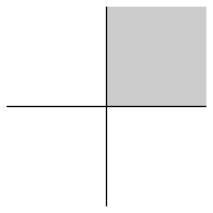
\includegraphics{3_a_subspaces_a.eps}} & \hspace{0.25in} &\begin{minipage}{0.2in} (b) \vspace{1.3in}\end{minipage} &\resizebox{!}{1.5in}{\includegraphics{3_a_subspaces_b.eps}} 
\end{tabular} \\
\begin{tabular}{llcclc} 
\begin{minipage}{0.2in} (c) \vspace{1.4in}\end{minipage} &\resizebox{!}{1.5in}{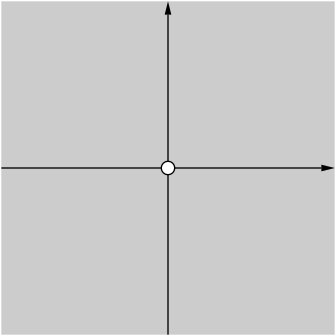
\includegraphics{3_a_subspaces_e.eps}} & \hspace{0.25in} &\begin{minipage}{0.2in} (d) \vspace{1.3in}\end{minipage} &\resizebox{!}{1.5in}{
\includegraphics{3_a_subspaces_g.eps}}
\end{tabular} %\\


\item Determine which of the following sets $W$ is a subspace of $\R^n$ for the indicated value of $n$. Justify your answer.

\ba
\item $W = \{[x \ 0]^{\tr} : x \text{ is a scalar}\}$
\item $W = \{[2x+y \ x-y \ x+y]^{\tr} : x,y \text{ are scalars}\}$
\item $W = \{[x+1 \ x-1]^{\tr} : x \text{ is a scalar}\}$
\item $W = \{[xy \ xz \ yz ]^{\tr} : x,y,z \text{ are scalars}\}$
\ea



\item Find a subset of $\R^2$ that is closed under addition and scalar multiplication, but that does not contain the zero vector, or explain why no such subset exists. 

\item Let $\vv$ be a vector in $\R^2$. What is the smallest subspace of $\R^2$ that contains $\vv$? Explain. Describe this space geometrically. 

\item What is the smallest subspace of $\R^2$ containing the first quadrant? Justify your answer. 

\item Let $\vu$, $\vv$, and $\vw$ be vectors in $\R^3$ with $\vw = \vu+\vv$. Let $W_1 = \Span\{\vu,\vv\}$ and $W_2 = \Span\{\vu,\vv,\vw\}$. 
\ba
\item If $\vx$ is in $W_1$, must $\vx$ be in $W_2$? Explain.

\item If $\vy$ is in $W_2$, must $\vy$ be in $W_1$? Explain.

\item What is the relationship between $\Span\{\vu,\vv\}$ and $\Span\{\vu,\vv,\vw\}$? Be specific. 

\ea

\item Let $m$ and $n$ be positive integers, and let $\vv$ be in $\R^n$. Let $W = \{A\vv : A \in \M_{m \times n}\}$. 
\ba
\item As an example, let $\vv = [2 \ 1]^{\tr}$ in $\R^2$ with $W = \{A\vv : A \in \M_{2 \times 2}\}$. 
	\begin{enumerate}[i.]
	\item Show that the vector $[2 \ 1]^{\tr}$ is in $W$ by finding a matrix $A$ that places $[2 \ 1]^{\tr}$ in $W$.  
	\item Show that the the vector $[4 \ 2]^{\tr}$ is in $W$ by finding a matrix $A$ that places $[4 \ 2]^{\tr}$ in $W$. 
	\item Show that the vector $[6 \ -1]^{\tr}$ is in $W$ by finding a matrix $A$ that places $[6 \ -1]^{\tr}$ in $W$. 
	\item Show that $W = \R^2$. 
	\end{enumerate}
	
\item Show that, regardless of the vector $\vv$ selected, $W$ is a subspace of $\R^m$. 

\item Characterize all of the possibilities for what the subspace $W$ can be. (Hint: There is more than one possibility.)

\ea

\item Let $S_1$ and $S_2$ be subsets of $\R^3$ such that $\Span \ S_1 = \Span \ S_2$. Must it be the case that $S_1$ and $S_2$ contain at least one vector in common? Justify your answer. 

\item Assume $W_1$ and $W_2$ are two subspaces of $\R^n$. Is $W_1 \cap W_2$ also a subspace of $\R^n$? Is $W_1 \cup W_2$ also a subspace of $\R^n$? Justify your answer. (Note: The notation $W_1 \cap W_2$ refers to the vectors common to both $W_1, W_2$, while the notation $W_1 \cup W_2$ refers to the vectors that are in at least one of $W_1, W_2$.)

\item Determine whether the plane defined by the equation $5x+3y-2z=0$ is a subspace in $\R^3$. 

\item If $W$ is a subspace of $\R^n$ and $\vu$ is a vector in $\R^n$ not in $W$, determine whether 
\[ \vu+W = \{\vu+\vv: \vv \text{ is a vector in }W\} \]
is a subspace of $\R^n$.

\item Two students are talking about examples of subspaces. 
\begin{quote}
Student 1: The $x$-axis in $\R^2$ is a subspace. It is generated by the vector $\left[ \begin{array}{c} 1\\0 \end{array}\right]$. 
\end{quote} 
\begin{quote}
Student 2: Similarly $\R^2$ is a subspace of $\R^3$. 
\end{quote} 
\begin{quote}
Student 1: I'm not sure if that will work. Can we fit $\R^2$ inside $\R^3$? Don't we need $W$ to be a subset of $\R^3$ if it is a subspace of $\R^3$?
\end{quote} 
\begin{quote}
Student 2: Of course we can fit $\R^2$ inside $\R^3$. We can think of $\R^2$ as vectors $\left[ \begin{array}{c} a\\b\\0 \end{array} \right]$. That's the $xy$-plane.
\end{quote} 
\begin{quote}
Student 1: I don't know. The vector $\left[ \begin{array}{c} a\\b\\0 \end{array} \right]$ is not exactly same as $\left[ \begin{array}{c} a\\b \end{array} \right]$. 
\end{quote}
\begin{quote}
Student 2: Well, $\R^2$ is a plane and so is the $xy$-plane. So they must be equal, shouldn't they? 
\end{quote} 
\begin{quote}
Student 1: But there are infinitely many planes in $\R^3$. They can't all be equal to $\R^2$. They all ``look like" $\R^2$ but I don't think we can say they are equal.
\end{quote}
Which student is correct? Is $\R^2$ a subspace of $\R^3$, or not? Justify your answer.

\item \label{ex:3_a_sum} Given two subspaces $H_1, H_2$ of $\R^n$, define 
\[ H_1+H_2 = \{ \vw \mid \vw=\vu+\vv \text{ where } \vu \text{ in }H_1, \vv \text{ in }H_2\} \,.\]
Show that $H_1+H_2$ is a subspace of $\R^n$ containing both $H_1, H_2$ as subspaces. The space $H_1+H_2$ is the sum\index{subspace!sum} of the subspaces $H_1$ and $H_2$.

\item Label each of the following statements as True or False. Provide justification for your response.
\ba
\item \textbf{True/False} Any line in $\R^n$ is a subspace in $\R^n$.

\item \textbf{True/False} Any line through the origin in $\R^n$ is a subspace in $\R^n$.

\item \textbf{True/False} Any plane through the origin in $\R^n$ is a subspace in $\R^n$.

\item \textbf{True/False} In $\R^4$, the points satisfying $xy=2t+z$ form a subspace.

\item \textbf{True/False} In $\R^4$, the points satisfying $x+3y=2z$ form a subspace.

\item \textbf{True/False} Any two nonzero vectors generate a plane subspace in $\R^3$.

\item \textbf{True/False} The space $\R^2$ is a subspace of $\R^3$.

\item \textbf{True/False} If $W$ is a subspace of $\R^n$ and $\vu$ is in $W$, then the line through the origin and $\vu$ is in $W$.

\item \textbf{True/False} There are four types of subspaces in $\R^3$: $\{\vzero\}$, line through origin, plane through origin and the whole space $\R^3$.

\item \textbf{True/False} There are four types of subspaces in $\R^4$: $\{\vzero\}$, line through origin, plane through origin and the whole space $\R^4$.

\item \textbf{True/False} The vectors $\left[ \begin{array}{c} 1\\1\\1 \end{array} \right]$, $\left[ \begin{array}{c} 1\\2\\1 \end{array} \right]$ and $\left[ \begin{array}{c} 2\\3\\2 \end{array} \right]$ form a subspace in $\R^3$.

\item \textbf{True/False} The vectors $\left[ \begin{array}{c} 1\\1\\1 \end{array} \right]$ and $\left[ \begin{array}{c} 1\\2\\1 \end{array} \right]$ form a basis of a subspace in $\R^3$.

\ea
\ee

\csection{Project: Least Squares Linear Approximation}
\label{sec:proj_ls_approx}

We return to the problem of finding the least squares line to fit the GDP-consumption data. We will start our work in a more general setting, determining the  method for fitting a linear function to fit any data set, like the GDP-consumption data, in the least squares sense. Then we will apply our result to the GDP-consumption data. 

\begin{pactivity} \label{act:ls_no_line} Suppose we want to fit a linear function $p(x) = mx+b$ to our data. For the sake of our argument, let us assume the general case where we have $n$ data points labeled as $(x_1,y_1)$, $(x_2, y_2)$, $(x_3, y_3)$,  $\ldots$, $(x_n, y_n)$. (In the GDP-consumption data $n = 21$.) In the unlikely event that the graph of $p(x)$ actually passes through these data points, then we would have the system of equations
\begin{align}
y_1 &= b + mx_1  \notag  \\
y_2 &= b + mx_2 \notag  \\
y_3 &= b + mx_3 \label{eq:LS_system} \\
\vdots &\hspace{0.39in} \vdots  \notag\\
y_n &= b + mx_n \notag
\end{align}
in the unknowns $b$ and $m$. 
	\ba
	\item As a small example to illustrate, write the system (\ref{eq:LS_system}) using the three points $(x_1,y_1)= (1,2)$, $(x_2,y_2) = (3,4)$, and $(x_3,y_3) = (5,6)$. Identify the unknowns and then write this system in the form $M \va = \vy$. Explicitly identify the matrix $M$ and the the vectors $\va$ and $\vy$.
	
	\item Identify the specific matrix $M$ and the specific vectors $\va$ and $\vy$ using the data in Table \ref{T:GDP_consumption}.  Explain why the system $M \va = \vy$ is inconsistent. (Remember, we are treating consumption as the independent variable and GDP as the dependent variable.) What does the result tell us about the data? 

	
	\ea

\end{pactivity}


Project Activity \ref{act:ls_no_line} shows that the GDP-consumption data does not lie on a line.  So instead of attempting to find coefficients $b$ and $m$ that give a solution to this system, which may be impossible, we instead look for a vector $\va^*$ that provides us with something that is ``close" to a solution.

If we could find $b$ and $m$ that give a solution to the system $M\va = \vy$, then $M\va - \vy$ would be zero. If we can't make $M\va - \vy$ exactly equal to the vector $\vzero$, we could instead try to minimize $M\va-\vy$ in some way. One way is to minimize the length $||M\va-\vy||$ of the vector $M\va - \vy$.

If we minimize the quantity $||M\va-\vy||$, then we will have minimized a function given by a sum of squares. That is, $||M\va-\vy||$ is calculated to be
\begin{equation}
 \sqrt{(b+mx_1-y_1)^2 + (b+mx_2-y_2)^2 + \cdots + (b+mx_n-y_n)^2}. \label{eq:ls_equation}
\end{equation}
This is why the method we will derive is called the method of least squares. This method provides us with a vector ``solution" in a subspace that is related to $M$. We can visualize $||M \va - \vy||$ as in Figure \ref{F:GDP_error}. In this figure the data points are shown along with a linear approximation (not the best for illustrative purposes). The lengths of the vertical line segments are the summands $(b+mx_i-y_i)$ in (\ref{eq:ls_equation}). So we are trying to minimize the sum of the squares of these line segments. 
\begin{figure}[ht]
\begin{center}
\resizebox{!}{2.5in}{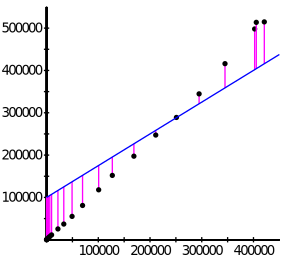
\includegraphics{GDP_error}}
\caption{Error in the linear approximation.}
\label{F:GDP_error}
\end{center}
\end{figure}

Suppose that $\va^*$ minimizes $||M \va - \vy||$. Then the vector $M \va^*$ is the vector that is closest to $\vy$ of all of the vectors of the form $M \vx$. The fact that the vectors of the form $M \vx$ make a subspace will be useful in what follows. We verify that fact in the next project activity.  

\begin{pactivity} \label{act:ls_subspace}  Let $A$ be an arbitrary $m \times k$ matrix. Explain why the set $C = \{A \vx : \vx \in \R^k\}$ is a subspace of $\R^m$. 


\end{pactivity}

Project Activity \ref{act:ls_subspace} shows us that even though the GDP-consumption system $M \va = \vy$ does not have a solution, we can find a vector that is close to a solution in the subspace $\{M \vx : \vx \in \R^2\}$. That is, find a vector $\va^*$ in $\R^{2}$ such that $M \va^*$ is as close (in the least squares sense) to $\vy$ as we can get. In other words, the error $||M \va^* - \vy||$ is as small as possible. In the following activity we see how to find $\va^*$. 

\begin{pactivity} \label{act:ls_minimum} Let 
\[S = \sqrt{(b+mx_1-y_1)^2 + (b+mx_2-y_2)^2 + \cdots + (b+mx_n-y_n)^2},\]
the quantity we want to minimize. The variables in $S$ are $m$ and $b$, so we can think of $S$ as a function of the two independent variables $m$ and $b$. The square root makes calculations more complicated, so it is helpful to notice that $S$ will be a minimum when $S^2$ is a minimum. Since $S^2$ is also function of the two variables $b$ and $m$, the minimum value of $S^2$ will occur when the partial derivatives of $S^2$ with respect to $b$ and $m$ are both $0$ (if you haven't yet taken a multivariable calculus course, you can just assume that this is correct). This yields the equations 
\begin{align}
0 &= \sum_{i=1}^n \left( mx_i + b - y_i\right)x_i  \label{eq:ls_1} \\
0 &= \sum_{i=1}^n \left( mx_i+b-y_i\right). \label{eq:ls_2}
\end{align}
In this activity we solve equations (\ref{eq:ls_1}) and (\ref{eq:ls_2}) for the unknowns $b$ and $m$. (Do this in a general setting without using specific values for the $x_i$ and $y_i$.)
	\ba
	\item Let $r=\sum_{i=1}^n x_i^2$, $s=\sum_{i=1}^n x_i$, $t = \sum_{i=1}^n y_i$, and $u = \sum_{i=1}^n x_iy_i$. Show that the equations (\ref{eq:ls_1}) and (\ref{eq:ls_2}) can be written in the form 
\begin{align*}
0 &= bs + mr -u \\ %\label{eq:revised_1} \\
0 &= bn + ms - t. %\label{eq:revised_2}.
\end{align*}	
Note that this is a system of two linear equations in the unknowns $b$ and $m$.

	\item Write the system from part (a) in matrix form $A \vx = \vb$. Then use techniques from linear algebra to solve the linear system to show that 
\begin{equation} \label{eq:ls_b} 
b = \frac{tr-us}{nr-s^2} = \frac{\left(\sum_{i=1}^n y_i\right) \left(\sum_{i=1}^n x_i^2\right) - \left(\sum_{i=1}^n x_i \right) \left(\sum_{i=1}^n x_iy_i \right)}{n\left(\sum_{i=1}^n x_i^2 \right) - \left(\sum_{i=1}^n x_i \right)^2}
\end{equation}
and
\begin{equation} \label{eq:ls_m} 
m = \frac{nu-ts}{nr-s^2} =  \frac{n\left(\sum_{i=1}^n x_iy_i\right) - \left(\sum_{i=1}^n x_i \right) \left(\sum_{i=1}^n y_i \right)}{n\left(\sum_{i=1}^n x_i^2 \right) - \left(\sum_{i=1}^n x_i \right)^2}.
\end{equation}


\ea

\end{pactivity}
 
\begin{pactivity} Use the formulas (\ref{eq:ls_b}) and (\ref{eq:ls_m}) to find the values of $b$ and $m$ for the regression line to fit the GDP-consumption data in Table \ref{T:GDP_consumption}. You may use the fact that the sum of the GDP data is $3.5164030 \times 10^6$, the sum of the consumption data is $2.9233750 \times 10^6$, the sum of the squares of the consumption data is $8.806564894 \times 10^{11}$, and the sum of the products of the GDP and consumption data is $1.069946378 \times 10^{12}$. Compare to the results the authors obtained in the paper  ``A Statistical Analysis of GDP and Final Consumption Using Simple Linear Regression, the Case of Romania 1990-2010". 



\end{pactivity}



